\section{Proof of semantic preservation}
\label{sec:proof}

The semantic preservation property of the HM2T is expressed by a
\textit{forward simulation} theorem, which general form is as follows
(according to \cite{Leroy2009}):
\begin{equation*}
  \forall{}S,C,B,\mathtt{transf}(S)=C\land{}S\Downarrow{}B\Rightarrow{}\exists{}B'~s.t.~C\Downarrow{}B'\land{}B\sim{}B'.
\end{equation*}

Considering the above theorem in a more general framework than the one
of compilers from programming languages (which is the framework of
\cite{Leroy2009}), $S$ corresponds to a source representation, and $C$
is the result of the transformation of $S$ by the transformation
function $\mathtt{transf}$; $B$ and $B'$ are behaviors, and the binary
relation $\Downarrow$ states that a given representation has a given
behavior. $B\sim{}B'$ states that the behavior $B$ is similar to the
behavior $B'$ considering a contextual definition of the similarity
relation. The forward simulation theorem must be read as follows: for
all source representation $S$ transformed into $C$ by function
$\mathtt{transf}$, if $S$ has a behavior $B$, then $C$ has a behavior
$B'$ that is similar to $B$. In our case, we have proved a slightly
different theorem, which has the following form:
\begin{equation*}
  \forall{}S,C,B,B',~\mathtt{transf}(S)=C\land{}S\Downarrow{}B\land{}C\Downarrow{}B'\Rightarrow{}B\sim{}B'.
\end{equation*}
In the above form, we consider that the target $C$ has the behavior
$B'$, and we no more have to prove the existence of such a behavior.
This version of the theorem focuses on the behavior similarity. In our
work perspectives, we contrive to prove the first form of the theorem,
but in this article we will present the proof of the second form.

In our specific transformation case, $S$ is a SITPN model and $C$ is a
\hvhdl{} design. The behavior of a SITPN model and a \hvhdl{} design
corresponds to the execution trace computed through a certain number
of clock cycles w.r.t. their respective semantics rules. Thus, the
property of semantic preservation for the HM2T is about the comparison
of the execution traces of the input SITPN model and the output
\hvhdl{} design. Specifically, we want to show that, no matter how
much clock cycles are performed, the execution traces are always
\textit{similar}. Figure~\ref{fig:trace-comparison} illustrates the
comparison of the execution traces of a SITPN model input of the HM2T
and its corresponding output design. 
\begin{figure}[!ht]
  \centering
  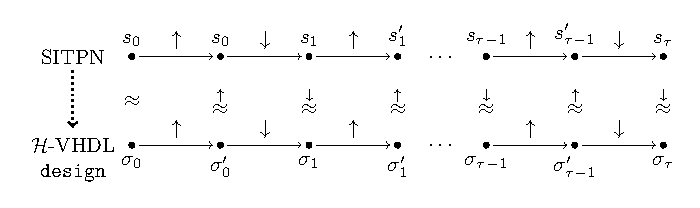
\includegraphics[keepaspectratio,width=\textwidth]{trace-comparison-full.eps}
  \caption{Comparison between the execution trace of a SITPN model (on
    the upper part) and the execution trace of the \hvhdl{} design
    resulting from the HM2T (on the lower part).}
  \label{fig:trace-comparison}
\end{figure}

In Figure~\ref{fig:trace-comparison}, $\tau$ indicates an arbitrary
number of clock cycles. To perform the proof of semantic preservation,
we must prove that every pair of states considered at the same time
point are similar w.r.t. to our own similarity relation.  Let us
introduce our general similarity criterions between a SITPN state and
a \hvhdl{} state through the relation presented in
Definition~\ref{def:state-sim}.

\begin{definition}[State similarity relation]
  \label{def:state-sim}
  For a given $sitpn\in{}SITPN$, a \hvhdl{} design $d\in{}design$, and
  a binder $\gamma\in{}WM(sitpn,d)$, an SITPN state $s\in{}S(sitpn)$
  and a design state $\sigma\in\Sigma$ are similar, written
  $\gamma\vdash{}s\approx\sigma$ if
  \begin{enumerate}
  \item\label{item:sim-mark} $\forall{}p\in{}P,$
    $~s.M(p)=\sigma(\gamma(p))($\texttt{s\_marking}$)$.
  \item\label{item:sim-tc}
    $\forall{}t\in{}T_i,$\\
    $\big(u(I_s(t))=\infty\land{}s.I(t)\le{}l(I_s(t))\Rightarrow{}s.I(t)=\sigma(\gamma(t))($\texttt{s\_time\_counter}$)\big)$\\
    $\land\big(u(I_s(t))=\infty\land{}s.I(t)>{}l(I_s(t))\Rightarrow{}\sigma(\gamma(t))($\texttt{s\_time\_counter}$)=l(I_s(t))\big)$\\
    $\land\big(u(I_s(t))\neq\infty\land{}s.I(t)>{}u(I_s(t))\Rightarrow{}\sigma(\gamma(t))($\texttt{s\_time\_counter}$)=u(I_s(t))\big)$\\
    $\land\big(u(I_s(t))\neq\infty\land{}s.I(t)\le{}u(I_s(t))\Rightarrow{}s.I(t)=\sigma(\gamma(t))($\texttt{s\_time\_counter}$)\big)$.
  \item\label{item:sim-reset} $\forall{}t\in{}T_i,$
    $s.reset_t(t)=\sigma(\gamma(t))($\texttt{s\_reinit\_time\_counter}$)$.
  \item\label{item:sim-cond}
    $\forall{}c\in\mathcal{C},~s.cond(c)=\sigma(\gamma(c))$.
  \item\label{item:sim-act}
    $\forall{}a\in\mathcal{A},~s.ex(a)=\sigma(\gamma(a))$.
  \item\label{item:sim-fun}
    $\forall{}f\in\mathcal{F},~s.ex(f)=\sigma(\gamma(f))$.
  \end{enumerate}
\end{definition}

In Definition~\ref{def:state-sim}, the binder structure $\gamma$ that
is generated by the HM2T relates the elements of the SITPN model to
the elements of the \hvhdl{} design, and thus enables the comparison
between a SITPN state and a \hvhdl{} state. In
Definition~\ref{def:state-sim}, Point~\ref{item:sim-mark} relates the
marking value of a place $p$ at state $s$ to the value of the
\texttt{s\_marking} signal, which is an internal signal of the PDI
identified by $\gamma(p)$. Here, the expression $\sigma(\gamma(p))$
returns the internal state of a PDI by looking up the component store
of state $\sigma$. Points~\ref{item:sim-tc} and \ref{item:sim-reset}
similarly relate the value of time counters (resp. reset orders) of
transitions to the value of the signals $\texttt{s\_time\_counter}$
(resp. $\texttt{s\_reinit\_time\_counter}$) in the internal state of
the corresponding TDIs. In Point~\ref{item:sim-cond}
(resp. \ref{item:sim-act} and \ref{item:sim-fun}), the Boolean value
of conditions (resp. actions and functions) are compared to the value
of input (resp. output) ports of the output design, also based on the
$\gamma$ binder.  As one can observe in Point~\ref{item:sim-tc}, due
to the specific implementation of time intervals with an infinite
upper bound in \hvhdl{}, the relation between the value of a time
counter and the value of the $\texttt{s\_time\_counter}$ signal can
not be restricted to a simple equality.

As shown in Figure~\ref{fig:trace-comparison}, we make a distinction
between the state similarity after a rising edge phase and after a
falling edge phase. The definitions of the post rising edge similarity
relation, written $\stackrel{\uparrow}{\approx}$, and the post falling
edge similarity relation, written $\stackrel{\uparrow}{\approx}$, are
restrictions of the general definition. After a rising edge phase, the
equality between the value of conditions and the value of condition
ports (i.e. Point~\ref{item:sim-cond} of
Definition~\ref{def:state-sim}) does not hold. And after a falling
edge phase, the equality between the value of time counter reset
orders and the value of the \texttt{srtc} signals
(i.e. Point~\ref{item:sim-reset} of Definition~\ref{def:state-sim})
does not hold. However, these divergences do not impact the
computation logic of the overall so that to create further behavioral
divergences between the input SITPN model and the output \hvhdl{}
design.


%%% Local Variables:
%%% mode: latex
%%% TeX-master: "main"
%%% End:
